\documentclass[conference]{IEEEtran}

\usepackage{cite}
\usepackage{amsmath,amssymb}
\usepackage{graphicx}
\usepackage{float}
\usepackage{booktabs}
\usepackage{array}
\usepackage{tabularx}
\usepackage{multirow}
\usepackage{tikz}
\usepackage{xcolor}
\usepackage{url}

\usetikzlibrary{arrows.meta,positioning}

\newcolumntype{Y}{>{\raggedright\arraybackslash}X}
\newcolumntype{L}[1]{>{\raggedright\arraybackslash}p{#1}}

\title{Estimating Final Load Capacity of Corroded Ferrocement Specimens From Metadata and Surface Corrosion Images}

\author{\IEEEauthorblockN{Parastoo Hashemi Alvar}
\IEEEauthorblockA{\textit{Politecnico di Torino} \\
s339438 \\
s339438@studenti.polito.it}
}

\begin{document}

\maketitle

\begin{abstract}

Visible corrosion is easy to observe, but the structural consequences of corrosion are much harder to measure directly. This creates a common problem in corrosion-related machine learning: image data are dense and repeated over time, while structural labels are sparse and often available only at the end of the experiment. Rather than attempting direct remaining-life prediction under these limitations, this study focuses on a narrower and more defensible question: can terminal ultimate load be estimated from specimen metadata and image-derived descriptors of surface corrosion? The analysis uses 791 aligned observations from 48 ferrocement specimens across two campaigns, with one measured terminal load value per specimen. To avoid optimistic bias, all evaluation is performed with specimen-level separation so that no specimen appears in both training and test sets. Three predictor families are compared: metadata, RGB-based visual descriptors, and HSV-based visual descriptors. Repeated grouped cross-validation, leave-one-campaign-out stress testing, mesh-stratified analysis, and post-onset sensitivity analysis are used to evaluate robustness. The best model for estimating final structural load capacity in the main grouped evaluation is a metadata-only Ridge regression model, achieving mean absolute error of 0.173~kN, root mean squared error of 0.214~kN, and Spearman correlation of 0.758. Adding image-derived corrosion descriptors does not provide a meaningful overall improvement in the combined dataset. However, image features become more competitive in later corrosion stages and within specific specimen groups. The study shows that visible corrosion is informative, but its contribution depends strongly on dataset structure and subgroup context.
\end{abstract}

\begin{IEEEkeywords}
corrosion assessment, ferrocement, structural capacity, image descriptors, grouped evaluation, regression
\end{IEEEkeywords}

\section{Introduction}
Visible corrosion is one of the earliest signs of structural deterioration. Rust patches, darker regions, and changes in color or texture can be recorded easily from images, which makes image-based corrosion analysis attractive for structural monitoring. The larger engineering question is whether these visible patterns might act as an indicator of deeper structural consequences.

In small experimental datasets, that question is not straightforward. Image observations are often repeated over time for each specimen, but structural measurements are sparse and often recorded only once at the terminal stage. Under these conditions, strong claims about hidden damage or remaining useful life can easily go beyond what the data actually support.

This study addresses that issue by deliberately narrowing the problem. Instead of asking whether images can predict full structural life, we ask whether they can improve the estimation of a directly measured terminal quantity: ultimate load. This reframing is central to the paper. It aligns the learning task with the strongest available structural evidence and allows a clearer comparison between engineering metadata and image-derived corrosion descriptors.

The paper addresses three questions:
\begin{enumerate}
    \item Can final structural load capacity be estimated from repeated observations collected during corrosion exposure?
    \item Do image-derived surface corrosion descriptors improve prediction beyond known specimen and exposure information?
    \item Do the conclusions remain the same when the data are examined within separate specimen groups rather than only in the full combined dataset?
\end{enumerate}

\begin{figure*}[t]
    \centering
    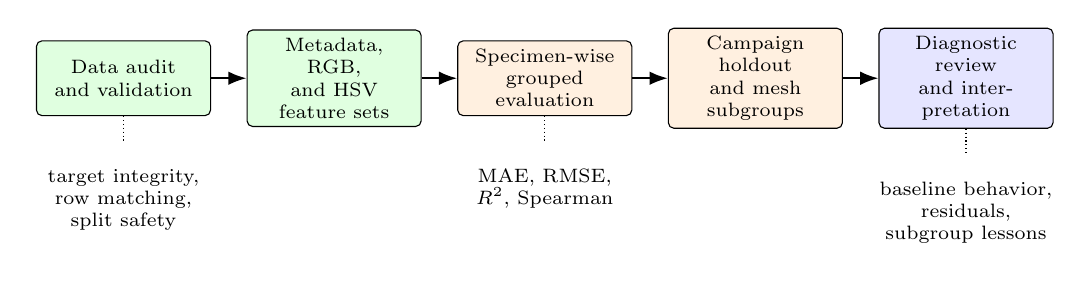
\begin{tikzpicture}[
        >=Latex,
        node distance=0.45cm,
        every node/.style={font=\scriptsize, align=center},
        stage/.style={draw, rounded corners=2pt, minimum height=0.95cm, text width=2.0cm, inner sep=3pt},
        observed/.style={stage, fill=green!12},
        analysis/.style={stage, fill=orange!12},
        result/.style={stage, fill=blue!10}
    ]
        \node[observed] (s1) {Data audit\\and validation};
        \node[observed, right=of s1] (s2) {Metadata, RGB,\\and HSV feature sets};
        \node[analysis, right=of s2] (s3) {Specimen-wise\\grouped evaluation};
        \node[analysis, right=of s3] (s4) {Campaign holdout\\and mesh subgroups};
        \node[result, right=of s4] (s5) {Diagnostic review\\and interpretation};

        \draw[->, thick] (s1) -- (s2);
        \draw[->, thick] (s2) -- (s3);
        \draw[->, thick] (s3) -- (s4);
        \draw[->, thick] (s4) -- (s5);

        \node[below=0.55cm of s1, text width=2.2cm] {target integrity, row matching, split safety};
        \node[below=0.55cm of s3, text width=2.2cm] {MAE, RMSE, $R^2$, Spearman};
        \node[below=0.55cm of s5, text width=2.2cm] {baseline behavior, residuals, subgroup lessons};

        \draw[densely dotted] (s1.south) -- ++(0,-0.32);
        \draw[densely dotted] (s3.south) -- ++(0,-0.32);
        \draw[densely dotted] (s5.south) -- ++(0,-0.32);
    \end{tikzpicture}
    \caption{Overview of the refocused workflow. The study first verifies the dataset and target definition, then compares metadata, RGB, and HSV predictor groups under specimen-wise grouped evaluation, subgroup analysis, and diagnostic review. The workflow is designed to answer whether image-derived corrosion descriptors improve estimation of final structural load capacity beyond known specimen information.}
    \label{fig:workflow}
\end{figure*}

\section{Study Reframing and Contributions}
This stage contributes more than a new model. First, it reframes the project around a measurable and defensible structural target. Second, it introduces an explicit audit and validation step before modeling. Third, it extends the visual representation by adding HSV-based descriptors and comparing them directly with RGB-based descriptors. Fourth, it evaluates models under specimen-wise splitting, group-wise analysis, campaign holdout, and a later-stage corrosion subset. Finally, it supports the main result with a diagnostic package rather than only average accuracy scores.

The paper therefore contributes both a predictive result and a more careful scientific interpretation of what the dataset can support.

\section{Data Audit and Predictor Design}
\subsection{Dataset and Validation}
The final dataset contains 791 usable observations from 48 specimens across two campaigns, covering 25 distinct week values from week 0 to week 36. Each observation combines specimen identity, time information, specimen and exposure properties, and one corresponding image. The structural target is the terminal ultimate load, available once per specimen, yielding 48 measured terminal outcomes.

The workflow began with an audit to confirm that the structural target, specimen identity, campaign labels, and image-table alignment were reliable enough for grouped evaluation. This audit also showed that the existing benchmark models and deterministic image feature extraction could be retained, but that the output structure needed to be expanded with manifests, split summaries, and organized diagnostics.

A key caution emerged during this review: campaign and mesh family were aligned in the dataset. This meant that pooled trends could be misleading and motivated the use of separate group-wise analyses.

\begin{table}[t]
    \caption{Dataset Summary}
    \label{tab:dataset}
    \centering
    \small
    \begin{tabular}{lr}
        \toprule
        Quantity & Value \\
        \midrule
        Usable observations & 791 \\
        Specimens & 48 \\
        Campaigns & 2 \\
        Week range & 0 to 36 \\
        Measured terminal load values & 48 \\
        Terminal measurements per specimen & 1 \\
        Specimens ending at week 28 & 24 \\
        Specimens ending at week 36 & 24 \\
        \bottomrule
    \end{tabular}
\end{table}

\subsection{Predictor Groups}
A central goal of the study was to determine whether visible corrosion contributes useful predictive information once specimen properties are already known. For that reason, the analysis did not begin by pooling all variables into a single model. Instead, several predictor groups were compared separately so that the study could distinguish among the signal carried by engineering metadata alone, image-derived descriptors alone, and their combinations.

\textbf{Metadata.} The metadata described specimen design and exposure conditions, including mesh count, chloride level, cover thickness, treatment group, specimen series, campaign, week, and ageing time. These variables formed the engineering baseline because they were available without image analysis and already encoded important differences in specimen configuration and exposure regime.

\textbf{RGB-based image descriptors.} The RGB-based descriptors summarized visible corrosion in the original image color space. They captured average color intensity, channel variation, brightness, grayscale histogram structure, texture, rust-covered area, dark and gray region ratios, morphology of corroded regions, and the spatial distribution of corrosion along the specimen. These features were included because visible corrosion first appears through changes in color, darkness, local concentration, and surface texture.

\textbf{HSV-based image descriptors.} The HSV-based descriptors represented the image in terms of hue, saturation, and brightness. They summarized channel means, within-channel variation, percentile values, and histogram distributions. This feature family was added in the refocused workflow because it allowed the study to compare two different visual representations of corrosion: RGB, which preserves the original image colors, and HSV, which separates color tone from brightness and intensity.

\textbf{Combined predictor groups.} Three mixed sets were also evaluated: metadata + RGB, metadata + HSV, and metadata + RGB + HSV. These combined models were central to the study because they tested whether visible corrosion descriptors improved prediction beyond the engineering baseline rather than simply performing well in isolation.

\begin{table}[t]
    \caption{Predictor Groups Used in the Study}
    \label{tab:predictors}
    \centering
    \small
    \begin{tabular}{L{0.33\linewidth}cL{0.4\linewidth}}
        \toprule
        Predictor Group & No. of Variables & Purpose \\
        \midrule
        Metadata & 11 & Engineering baseline \\
        RGB image descriptors & 41 & Surface corrosion in original color space \\
        HSV image descriptors & 36 & Surface corrosion in alternative color space \\
        Metadata + image combinations & up to 88 & Test added value of visible corrosion \\
        \bottomrule
    \end{tabular}
\end{table}

\section{Experimental Protocol}
The prediction task in this paper is estimating final structural load capacity. All reported best models refer to that task.

Five regression models were compared: Ridge Regression, Random Forest, Gradient Boosting, XGBoost, and CatBoost. The main evaluation used specimen-wise train-test separation, meaning that all rows from a specimen were kept together so that the model never trained on one time point of a specimen and tested on another time point of the same specimen.

Four evaluation views were used:
\begin{itemize}
    \item the main grouped evaluation across all specimens,
    \item a campaign-holdout stress test,
    \item separate analyses for the 4-mesh and 7-mesh groups,
    \item and a later-stage corrosion subset that retained only observations after visible corrosion had clearly started.
\end{itemize}

In addition to model scores, the workflow generated out-of-fold predictions, residual plots, fold-stability summaries, uncertainty views based on repeated splits, and feature-importance summaries. A residual-refinement follow-up based on specimen-level summaries was also tested.

The main performance measures were mean absolute error (MAE), root mean squared error (RMSE), coefficient of determination ($R^2$), and Spearman correlation.

\begin{figure*}[t]
    \centering
    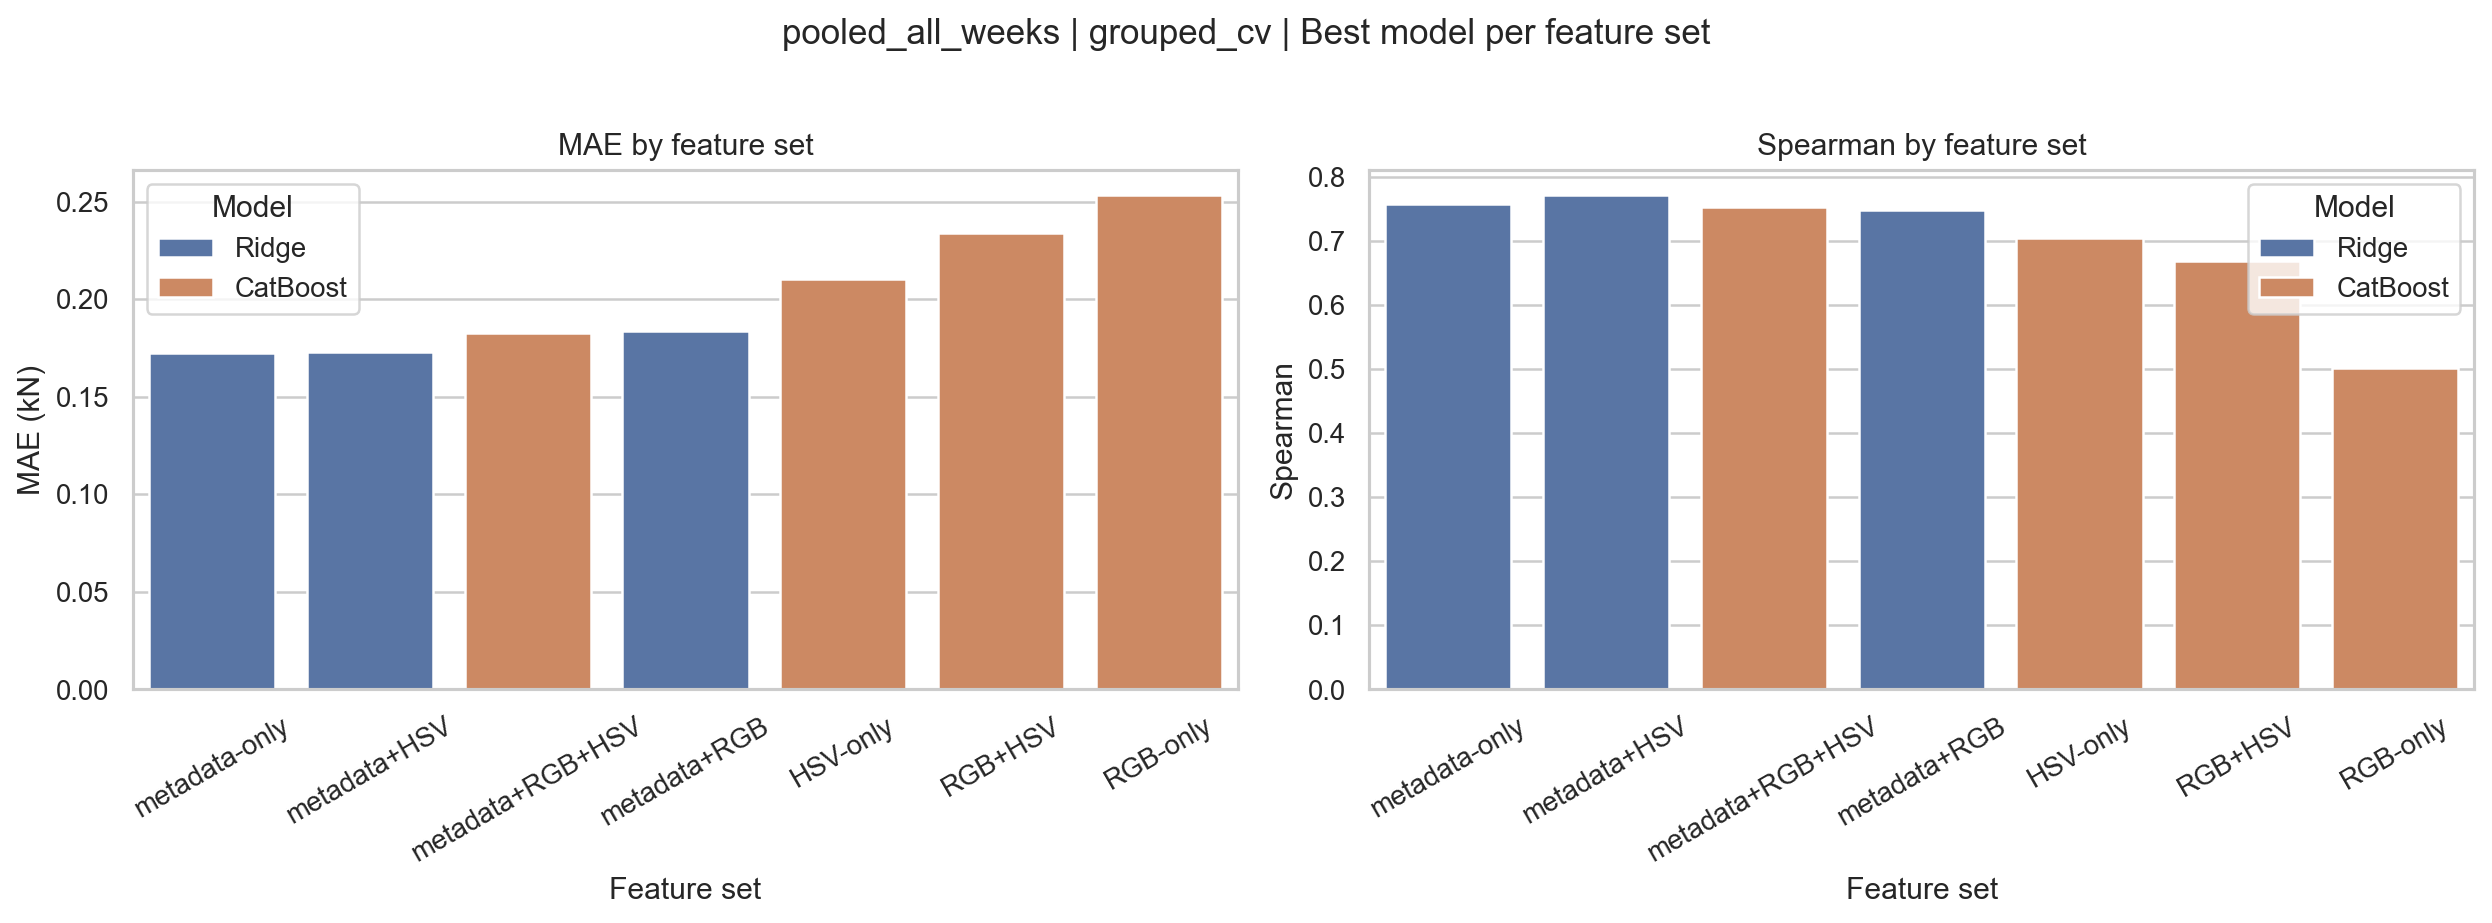
\includegraphics[width=0.96\textwidth]{../ultimate_load_refocus/pooled_all_weeks/grouped_cv/feature_set_comparison_bars.png}
    \caption{Grouped-evaluation comparison of the best model within each feature set. The left panel shows MAE and the right panel shows Spearman correlation. The figure highlights the central quantitative result of the study: metadata-only Ridge is the strongest overall baseline, while adding image-derived descriptors does not materially improve the pooled main setting.}
    \label{fig:feature-comparison}
\end{figure*}

\section{Results}
\subsection{Main Combined-Dataset Result}
The best model for estimating final structural load capacity in the main grouped evaluation was a metadata-only Ridge regression model. It achieved MAE $= 0.173 \pm 0.046$~kN, RMSE $= 0.214 \pm 0.054$~kN, $R^2 = 0.645 \pm 0.171$, and Spearman $= 0.758 \pm 0.205$.

The strongest non-baseline alternative was metadata + HSV with Ridge, but its performance was essentially unchanged relative to metadata only. This showed that visible corrosion descriptors did not provide a meaningful overall improvement in the combined dataset.

\subsection{Subgroup and Sensitivity Results}
The broader analysis showed that the role of image-derived information depended on context.

Within the 4-mesh group, the best model for estimating final structural load capacity was the metadata + RGB + HSV CatBoost model, with MAE of 0.194~kN. Within the 7-mesh group, the best model was the HSV-only CatBoost model, with MAE of 0.137~kN. In the later-stage corrosion subset, the best model was the metadata + RGB + HSV CatBoost model, with MAE of 0.163~kN, while metadata-only remained highly competitive at 0.173~kN.

The campaign-holdout stress test was much harder. In that setting, the best model for estimating final structural load capacity was a metadata-only Gradient Boosting model with MAE of 0.465~kN.

\begin{table*}[t]
    \caption{Key Results for Estimating Final Structural Load Capacity}
    \label{tab:key-results}
    \centering
    \small
    \begin{tabular}{L{0.25\linewidth}L{0.18\linewidth}L{0.16\linewidth}cccc}
        \toprule
        Evaluation Setting & Best Predictor Group & Best Model & MAE (kN) & RMSE (kN) & $R^2$ & Spearman \\
        \midrule
        Main grouped evaluation & Metadata only & Ridge & 0.173 & 0.214 & 0.645 & 0.758 \\
        Strongest non-baseline in main grouped evaluation & Metadata + HSV & Ridge & 0.173 & 0.215 & 0.635 & 0.771 \\
        4-mesh subgroup & Metadata + RGB + HSV & CatBoost & 0.194 & 0.238 & -0.998 & 0.081 \\
        7-mesh subgroup & HSV only & CatBoost & 0.137 & 0.174 & -0.386 & 0.460 \\
        Later-stage corrosion subset & Metadata + RGB + HSV & CatBoost & 0.163 & 0.208 & 0.660 & 0.791 \\
        Campaign-holdout stress test & Metadata only & Gradient Boosting & 0.465 & 0.503 & -4.639 & 0.217 \\
        \bottomrule
    \end{tabular}
\end{table*}

\subsection{Pooled vs Group-Wise Interpretation}
The correlation analysis reinforced the same message. When all specimens were combined, visible corrosion appeared positively associated with final load. However, once the 4-mesh and 7-mesh groups were analyzed separately, that pattern weakened sharply and often changed direction. This indicated that pooled trends were influenced by differences between specimen groups and should not be interpreted on their own.

\begin{figure}[t]
    \centering
    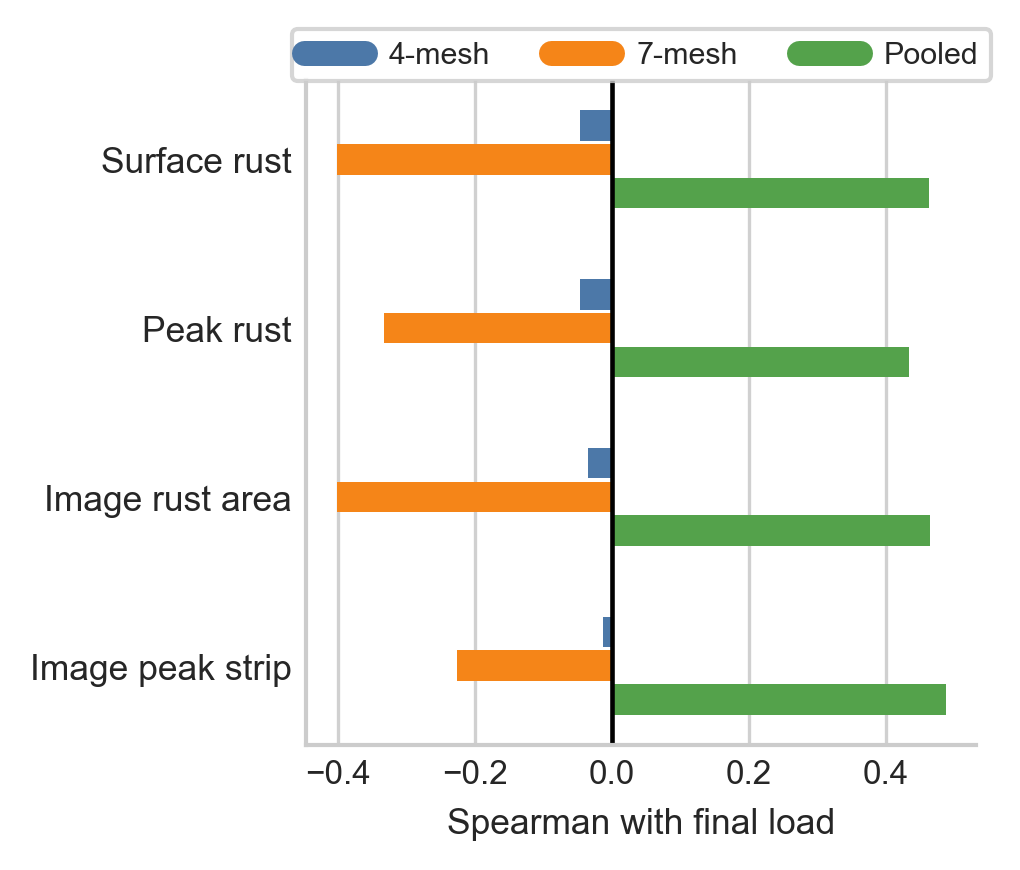
\includegraphics[width=\columnwidth]{../ultimate_load_refocus/correlations/mesh_stratified_spearman_summary.png}
    \caption{Spearman correlation between representative corrosion variables and final structural load capacity in pooled and mesh-stratified views. The pooled correlations are consistently positive, while the 4-mesh and 7-mesh correlations are weak or negative. This compact summary supports the paper's main interpretation that pooled corrosion-load trends are confounded by specimen-group structure.}
    \label{fig:mesh-stratified-correlation}
\end{figure}

\subsection{Diagnostic Findings}
The diagnostic package supported the stability of the main result. Out-of-fold predictions and residual views showed that the metadata baseline performed consistently across repeated grouped splits. The residual-refinement follow-up did not improve the metadata baseline, which strengthened confidence in the simpler model rather than replacing it with a more complex alternative. Feature-importance review also showed that the dominant signals in the combined dataset came from specimen-level engineering variables such as campaign, mesh count, cover thickness, and chloride level. A prediction-versus-ground-truth view of the selected baseline further clarified the same pattern: the model tracked the middle of the load range reasonably well, but compressed the lowest and highest terminal capacities toward the center.

\begin{figure}[H]
    \centering
    
\includegraphics[width=\columnwidth]{../ultimate_load_refocus/pooled_all_weeks/grouped_cv/experiments/metadata_only/Ridge/prediction_vs_ground_truth.png}
    \caption{Prediction-versus-ground-truth diagnostic for the metadata-only Ridge baseline in the main grouped evaluation. The dashed 1:1 line indicates perfect agreement between observed and predicted terminal load. The figure shows that the baseline follows the middle of the load range reasonably well but tends to overpredict the weakest specimens and underpredict the strongest ones, consistent with regression-to-the-mean behavior.}
    \label{fig:diagnostics}
\end{figure}

\section{Discussion}
The most important result is not simply that metadata-only Ridge achieved the lowest pooled MAE. The more important result is that, in this dataset, final structural load capacity is governed first by specimen design and exposure regime, and only second by what is visible at the surface. Variables such as mesh family, campaign, cover thickness, chloride level, and treatment already encode much of the between-specimen variation in terminal load. This explains why the metadata baseline was difficult to beat in the main grouped evaluation and why adding RGB or HSV descriptors produced little aggregate improvement in the pooled setting.

At the same time, the image should not be interpreted as irrelevant. The subgroup and later-stage analyses show a more specific role for visible corrosion descriptors: they become more useful once comparisons are made within more homogeneous specimen groups, or once corrosion is sufficiently developed to be clearly expressed at the surface. In other words, the image is not a universal replacement for engineering metadata, but a conditional source of additional signal whose value depends on when the specimen is observed and which specimens are being compared.

The strongest methodological lesson concerns interpretation. Because campaign and mesh family were aligned, pooled corrosion-load trends were partly driven by specimen-group structure rather than by a single monotonic corrosion-capacity relationship. The stratified correlation analysis and the severe campaign-holdout drop both support the same conclusion: without grouped splits and subgroup analysis, the study could easily have overstated the role of visible corrosion. The main contribution of the refocused workflow is therefore not only a useful terminal-load estimator, but also a clearer demonstration of how dataset structure governs what can and cannot be inferred from corrosion images.

\section{Limitations}
This study has several limitations. First, final structural load capacity was measured only once per specimen, so the task was terminal-load estimation rather than full structural-history modeling. Second, campaign and mesh family were aligned, which complicated pooled interpretation and made campaign holdout a severe extrapolation test. Third, although the dataset included many repeated observations, the structural supervision still came from only 48 terminal measurements. Finally, the image features described visible surface condition only; they did not directly measure hidden internal deterioration.

\section{Conclusion}
This paper presented a refocused and more defensible study of corrosion-related structural prediction. Instead of targeting a broader life quantity, it examined whether final structural load capacity could be estimated from repeated observations of corroded ferrocement specimens.

The workflow combined data audit, metadata and image-feature comparison, specimen-wise evaluation, subgroup analysis, later-stage sensitivity analysis, and diagnostic review. The best model for estimating final structural load capacity in the main grouped evaluation was a metadata-only Ridge regression model with MAE of 0.173~kN and Spearman correlation of 0.758. Image-derived corrosion descriptors did not provide a meaningful overall improvement in the combined dataset, but they became more competitive within specific specimen groups and later corrosion stages.

The main conclusion is therefore twofold: final structural load capacity can be estimated with useful accuracy, and the value of visible corrosion depends strongly on dataset structure and subgroup context. In the combined dataset, specimen properties dominate. In more specific settings, image-derived corrosion information becomes more relevant.

\end{document}
